\documentclass[10pt]{article}
%%%%%%%%%%%%%%%%%%%%%%%%%%%%%%%%%%%%%%%%%%
%                   ┌┐  ┌┐
%                   ││  ││
%┌──┐┌─┐┌──┐┌──┐┌┐┌┐│└─┐││ ┌──┐
%│┌┐││┌┘││─┤│┌┐││└┘││┌┐│││ ││─┤
%│└┘│││ ││─┤│┌┐││││││└┘││└┐││─┤
%│┌─┘└┘ └──┘└┘└┘└┴┴┘└──┘└─┘└──┘
%││
%└┘
%%%%%%%%%%%%%%%%%%%%%%%%%%%%%%%%%%%%%%%%%%
\usepackage[margin={1.8cm,1.8cm},top=2cm, bottom=2cm]{geometry}
\usepackage{amsmath} %for math equations and formality (like. \text{})
\usepackage{multicol} % multiple column package
\usepackage{authblk}
\usepackage{afterpage} % hacky page geometry
\usepackage{graphicx}
\usepackage{mwe}
\usepackage{indentfirst}
\usepackage{lmodern}
\usepackage{pgfplots} % for graphing (page 5 on the official document)
\usepackage{etoolbox}
\usepackage{tabularx}
\usepackage{changepage}
\usepackage{mathptmx} %font
\usepackage{bold-extra} % for titles
\usepackage{authblk} % több author címke
\usepackage{fancyhdr} % for nicer header
\pagestyle{fancy}
%%%%%%%%%%%%%%%%%%%%%%%%%%%%%%%%%%%%%%%%%%
\renewcommand{\headrulewidth}{0pt} % sets both header and footer to nothing
\fancyhf{} % removes numbering from the bottom of the page
\fancyhead[R]{\thepage}
% Roman numerals for numbering
\renewcommand{\thesection}{\sc{\Roman{section}}.} % Use roman numerals instead
\renewcommand\thesubsection{\Alph{subsection}} % use A,B,C ...
\renewcommand{\abstractname}{} % clear the title for abstract
\makeatletter
\title{\vspace{-4em} \fontfamily{ptm} \bfseries \Large Fractional Marcus-Hush-Chidsey-Yakopcic current-voltage model for redox-based resistive memory devices}
\date{(Dated: February 21, 2023)}
\makeatother
%%%%%%%%%%%%%%%%%%%%%%%%%%%%%%%%%%%%%%%%%%
\author[1]{Georgii Paradezhenko}
\author[1]{Dmitrii Prodan}
\author[1]{Anastasiia Pervishko}
\author[1]{Dmitry Yudin}
\author[2, 3]{Anis Allagui}
\affil[1]{\textit{Skolkovo Institute of Science and Technology, Moscow 121205, Russia}}
\affil[2]{\textit{Department of Sustainable and Renewable Energy Engineering, University of Sharjah, Sharjah, P.O. Box 27272, United Arab Emirates}}
\affil[3]{\textit{Department of Mechanical and Materials Engineering,
Florida International University, Miami, FL33174, United States}\vspace{-1em}}
%%%%%%%%%%%%%%%%%%%%%%%%%%%%%%%%%%%%%%%%%%
%┌──┐ ┌───┐┌───┐┌┐  ┌┐
%│┌┐│ │┌─┐│└┐┌┐││└┐┌┘│
%│└┘└┐││ ││ ││││└┐└┘┌┘
%│┌─┐│││ ││ ││││ └┐┌┘
%│└─┘││└─┘│┌┘└┘│  ││
%└───┘└───┘└───┘  └┘
%%%%%%%%%%%%%%%%%%%%%%%%%%%%%%%%%%%%%%%%%%
\begin{document}
\vspace{-1em}
% Showcase title on the page
\maketitle
%%%%%%%%%%%%%%%%%%%%%%%%%%%%%%%%%%%%%%%%%%
% Skip first-page numbering
\thispagestyle{empty}
%%%%%%%%%%%%%%%%%%%%%%%%%%%%%%%%%%%%%%%%%%
\begin{adjustwidth}{50pt}{50pt}
We propose a circuit-level model combining the Marcus-Hush-Chidsey electron current equation and the Yakopcic equation for the state variable for describing resistive switching memory devices of the structure metal–ionic conductor–metal. We extend the dynamics of the state variable originally described by a first-order time derivative by introducing a fractional derivative with an arbitrary order between zero and one. We show that the extended model fits with great fidelity the current-voltage characteristic data obtained on a Si electrochemical metallization memory device with Ag-Cu alloy.
\end{adjustwidth}
%%%%%%%%%%%%%%%%%%%%%%%%%%%%%%%%%%%%%%%%%%
% Set space between two columns
\setlength{\columnsep}{0.8cm}
%%%%%%%%%%%%%%%%%%%%%%%%%%%%%%%%%%%%%%%%%%
\begin{multicols}{2}
{\centering % Only center the section title
\section{\sc{introduction}}}
Substantial research efforts have been dedicated to the development of electrically-controlled resistive switching in metal-insulator-metal (MIM) devices or memristors, going from new materials discovery to modelling and simulation, and design and applications. With both memory and logic capabilities combined at the hardware level, in addition to long retention times and high switching rates at relatively low energy consumption, these devices are favorably seen as the next-generation building blocks for nonvolatile memories and neuromorphic computing applications. In a typical memristor, the resistive switching is based on the electrically-stimulated change of cell resistance usually driven by internal ion redistribution, which actually depends not only on the applied excitation but also on the past history of the excitation. Physical mechanisms associated with these reversible transitions have been attributed to different effects including valencechange, electrochemical metallization, and phase change effects. They can be either abrupt (binary) or gradual (analogue), and evolve at different timescales, leading to rich and complex device behaviors in this seemingly simple device structure of just three layers. Furthermore, with the wide range of diversity in memristors materials and their morphologies, operating mechanisms, and manufacturing technologies there is an urgent need for the development of a general model capable of capturing accurately and effectively their complex nonlinear dynamics. This is crucial not only for the characterization and comparison between different memristor devices, but also for the investigation of larger scale memristorbased circuits and hybrid hardware architectures, and also to explore similar behaviors observed for instance in biological synapse systems.
\par
While models at different size scales and thus with different degrees of physical details and computational complexity have been developed for memritors, including but not limited to ab initio, Kinetic Monte Carlo, and finite element method modells, in this work we focus on the circuit-level (compact) current-voltage behavior of the memristors. From this point of view, Memristors are generally described by the systems of coupled equations: 
\begin{align}
     i &= G(v,x)v, \\
     \dot{x} &= f(x,v),
\end{align}
where $i = i(t)$ is the current through the device, $v = v(t)$
is the applied voltage, and $x = x(t)$ corresponds to a state
variable or a group of state variables that quantify the
internal dynamics of the device. These are, for example,
width of doping region, concentration of vacancies in the gap region, and tunneling barrier width. State vairables can not be observed from external electrical behavior. Eq1. (1) follows the $i-v$ curve of the resistive device in the question with $G(v,x)$ being the generalized conductance, whereas Eq. describes the dynamics of the it's internal state x based on it's prehistory. The actual stat of a memristor can only be determined by solving Eqs. (1) and (2) self-consistently. Memristive systems as featured
in terms of Eqs. (1) and (2) are known to possess a pinched hysteresis loop at the origin in the i-v plane in the response to any periodic voltage source. \par
Being versatile and modular enough it is the Yakopcic model 27–29 which is most often used to simulate
the nonlinear i-v characteristic of wide range of memristors in response to sinusoidal and repetitive sweeping
inputs. The model takes into account electron transmission effects, voltage threshold for state variable motion,
and nonlinear velocity function for oxygen vacancies or
dopant drift, considered to be the most relevant internal
state information29. It follows on the steps of Strukov et
al. work30, and describes the memristor as two resistors
in series characterized by electron transmission equations
so that:
\begin{align}
     i(t) = h_1 (v)x + h_2 (v)(1-x) .
\end{align}
Here, h1 is used to model the behavior in the low resistance state of the device, and h2 captures its behavior in the high-resistance state.
The two electron transmission equations are weighted and mixed by the state
variable x which is set to take values between zero and
one25. In memristive devices, it is the rate of change of
the state variable x that is explicitly determined (2), and
is given in the Yakopcic memristor model by the product
of the two composite functions g(v) and f(x) such that29:
\begin{align}
     \dot{x} = g(v)f(x).
\end{align}
An exponential dependency of the state change to the
positive and negative regions of the input voltage v is
modelled in terms of
\begin{align}{}
     g(v) = \begin{cases} a_p \cdot (1-e^{U_p -v}) \cdot e^v, &u-u_p > 0, \\ a_n \cdot (e^{u_n +v}-1)\cdot e^{-v}, &u+u_n < 0, \\
     \centering 0, &\text{otherwise}\end{cases}
\end{align}
including programming voltage thresholds up and un.
The magnitude of state change for a voltage potential
is defined with ap and an. The second function f(x) is
determined by
\begin{align}
    f(x) = \begin{cases} w_p (x, x_p) \cdot e^{-(x-x_p), &x \ge x_p, \\
    1 &x < x_p,}\end{cases}
\end{align}
for $v > 0$, while $v < 0$, it is defined as
\begin{align}
    f(x) = \begin{cases} w_n (x, x_n) \cdot e^{x+x_n-1), &x \le x_n, \\
    1 &x > x_n,}\end{cases}
\end{align}
Effectively, this function introduces the nonlinear ion motion, as it becomes harder to change the state of the
devices when the state variable approaches the boundaries. In Eq. (6), $w_p(x, x_p)$ is a windowing function that
ensures $f(x)$ equals zero when $x(t) = 1$, and in (7),
$w_n(x, x_n)$ keeps $x(t)$ from becoming less than 0 when
the current flow is reversed. These two functions can explicitly be written as $w_p(x, x_p) = 1 + (x_p - x)/( 1 - x_p)$
and $w_n(x, x_n) = x/(1 - x_n)$. \par
Clearly, in (3), the functions h1 and h2 are dependent on the structure and type of memristor under study.
Several types of resistive switching memory devices can
be classified as nanoionic-based electrochemical systems,
wherein an ion conductor in the form of electron insulator layer is placed between two electrodes31,32. For the
case of cation-migration-based electrochemical metallization memory cells, Ag or Cu are typically used as active
electrodes, Pt or W as counter electrodes, and a variety
of oxides or chalcogenides thin films as solid electrolytes.
When a positive voltage is applied, the active electrode
material is oxidized at the electrode–electrolyte interface
leading to the release of metallic ions in the adjacent electrolyte, followed by drift and diffusion of these ions across
the electrolyte, and then their deposition in filamentarylike metal structures at the counter electrode surface.
Short-circuit occurs when the filament has grown sufficiently far to make an electronic contact with the opposite electrode, which defines the low-resistance state of
the cell. When a negative voltage is applied, the cell returns back, in principle reversibly, to the high-resistance state31. Anion-migration-based valence change cells, on
the other hand, are formed by placing a metal oxide
between for example Pt or TiN electrodes and another
oxygen-affine, lower work function electrode. The lowresistance and high-resistance states are defined based on
the electrochemical formation of oxygen-deficient, mixed
ionic–electronic conducting filaments, and the nanoionic
modification of the potential barrier between the tip of
the filament and the electrode it faces31. For these types
of redox-based resistive memory cells, it is more appropriate to consider electron transfer theory associated with
the kinetics of redox reactions to better describe their i-v
characteristics. Furthermore, because the formation and
rupture of the metallic filaments follow random paths,
the possibility of charge trapping from one operation sequence to another, charge leakage, the dynamics of an
internal state variable associated with these cells cannot
be defined solely based on its immediate past, in other
words via integer-order derivative as in (2). Taking into
account the integral past is believed to be more representative for a proper mathematical description of the
complexity and dissipative nature of these cells.
\par 
Motivated by these observations, we herein propose
a circuit-level model for redox-based resistive memory
devices, where the current equation (1) is taken from
the Marcus-Hush-Chidsey (MHC) theory33–35 of heterogeneous electron transfer, while the state variable equation (2) is taken from the Yakopcic generalized memristive model27. We consider the dynamics of the state variable with respect to time to be of fractional, non-integer,
order. Mathematically, this adds an extra degree of freedom to the model that can be generically correlated to
the non-perfect reversibility of the device when looking
at it from one cycle to another. We fit the extended
model to the experimental data obtained on a Si memristor with Ag-Cu alloy as reported in36. A close inspection
of numerical results unambiguously reveals that switching to the fractional derivative allows one to significantly
improve the agreement between the theory and experimental data.
{\centering % Only center the section title
\section{\scshape Memristor model}
}
The generalized i-v relationship, as specified by Eq. (1), for the proposed memristor model reads
\begin{align}
    i = \gamma _1 x h(\delta _1 v) + \gamma _2(1 - x) h (\delta _2 v),
\end{align}
where $\delta _1, \delta _2, \gamma _1, \gamma _2 > 0$ are model parameters, and the function
\begin{align}{}
    h (v) = h_+ (v) - h_- (v),
\end{align}
is based on the MHC model for electron transfer described by the Gauss-Fermi integral,
\begin{align}
    h_\pm (v) = \beta \int_{-\infty}^\infty = \exp{\biggl\{ -\frac{(z - \lambda \pm v)^2}{4 \lambda} \biggr\} } \frac{\,dz}{1+e^z}.
\end{align}
Here, the $\pm$ signs refer to the oxidative and reductive
transition rate functions, $\lambda$ is the dimensionless reorganization energy scaled to kBT, while the integral over the
dimensionless variable z accounts for the Fermi statistics of electron energies, distributed around the electrode
potential. The prefactor $\beta$ accounts for the electronic
coupling strength and the electronic density of states of
the electrode. In Eq. (10), $\lambda$ and $\beta$ are assumed to be
fitting parameters, knowing that $\beta$ is usually expressed
as an exponential term itself that depends on the distance between the donor and acceptor of electrons. This,
however, does not affect the generality of the proposed
model. Finally, v in Eqs. (8)–(10) is actually the electrochemical overpotential defined as the difference between
the equilibrium Nernst-potential of the metal and the
actual electrode potential defined by the external power
supply. We will consider the equilibrium potential to be
negligible, so that the electrochemical potential is equal
to the applied voltage on the device \par
For the dynamics of the state variable $x(t)$, we introduce a fractional time derivative in (4) as follows
\begin{align}
    D_t^\alpha = g(v)f(x), ~~~x(0) = x_0,
\end{align}
where $ D_t^\alpha$ is the fractional derivative operator of order
$\alpha > 0$ in the sense of Caputo
\begin{align}
    D_t^\alpha x(t) = \frac{1}{\Gamma (n-\alpha)} \int_0^t \frac{x^{(n)} (\tau)d \tau}{(t - \tau)^{\alpha+1-n}},
\end{align}
where $n-1<\alpha<n$, while $\Gamma (z)= \int_0^\infty t^{z-1} e^{-t} \,dt$ in the denominator stands for the Gamma function, and $x^{(n)} (\tau)$ is the n-th order derivative. In our follow-up study, the order of the derivative is assumed to be $0 < \alpha < 1$. \par
Thus the parameters
\begin{align}
    p = (\alpha, x_p, x_n, a_p, a_n, u_p, u_n, \beta, \lambda, \gamma _1, \gamma _2, \delta_1, \delta_2).
\end{align}
being arranged into one vector specify the proposed memristor model.
{\centering % Only center the section title
\section{\scshape methods}
}
{\centering \subsection{Evaluation of the MHC integral}}
The Gauss-Fermi integrals like (10) can be evaluated
numerically using the Gauss-Hermite quadrature (see,
e.g.,37). In practice
\begin{align}
    \int_{- \infty}^\infty e^{-x^2} f(x) \,dx \approx \sum_{k=1}^n c_k f(x_k),
\end{align}
where $n$ corresponds to the amount of sample points, while $x_k$ are the roots of the Chebyshev-Hermite polynomial $H_n (x_k) = 0$ with $k=1,...,n$. For a given $n \ge 2$ the Chebyshev-Hermite polynomial $H_n (x)$ can be identified
from recurrence relations
\begin{align}
    H_{n+1}(x) = 2xH_n(x) - 2nH_{n-1}(x),
\end{align}
provided $H_0(x)=1$ and $H_1(x) = 2x$. In (14), the coefficients $c_k$ are given by
\begin{align}
    c_k = \frac{2^{n-1}}{n^2} \frac{n!}{|H_{n-1 (x_k)}|^2} \sqrt{\pi},
\end{align}
Thus, one can rewrite the MHC integrals (10) in the form
\begin{align}
    h_{\pm}(v)=2 \beta \sqrt{\lambda} \sum_{k=1}^n \frac{c_k}{1+\exp{\{2x_k \sqrt{\lambda} + \lamda \pm v\}}}.
\end{align}
In our numerical simulations, the order of quadrature
$n = 25$, which is deemed more than sufficient for our purpose.
{\centering \subsection{Solution to the fractional differential equation}}
The nonlinear fractional differential equation (11)
is solved numerically using the Adams-type predictor corrector method38. For nonlinear fractional differential equations of the form
\begin{align}
    D_t^\alpha x(t) = F(t,x), ~~~ x^{(k)}(0) = x_0^{(k)},
\end{align}
where $k = 0, 1, . . . , m - 1$ and $m = [\alpha]$, this method can
be described as follows. The approach is based on the
fact that the initial value problem is equivalent to the
Volterra integral equation
\begin{align}
    x(t) = \sum_{k=0}^{m-1} \frac{t^k x_0^{(k)}}{k!} + \frac{1}{\Gamma (\alpha)} \int_0^t \frac{F(\tau , x(\tau))}{(t- \tau)^{1-\alpha}}
\end{align}
We assume that the choice of $F(t, x)$ guarantees the existence of a unique solution in a certain interval $0 \le t \le T$.
We divide this interval into $N$ equal pieces as specified
by a uniform grid at the points $t_n = hn, n = 0, 1, . . . , N$
and $h = T / N$. The basic idea is that using pre-calculated
approximations $x_h(t_j ) \approx x(t_j ), j = 0, 1, . . . , n$, we get
the next time step approximation $x_h(t_{n+1})$ by means of
Eq. (19). \par
Replacing the integral on the right-hand side of
Eq. (19) by the product rectangle rule, we obtain
\begin{align}
    \int_0^{t_{n+1}} \frac{F(\tau , x(\tau))}{(t_{n+1}-\tau)^{1-\alpha}}d\tau \approx \frac{h^\alpha}{\alpha} \sum_{j=0}^n F_j \cdot b_{n-j},
\end{align}
where $F_j = F(t_j , x_h(t_j))$ and $b_k = (k + 1)^\alpha - k^\alpha$
, provided that $0 \le k \le n$. The predicted value $x^P (t_{n+1})$ is
determined by the fractional Adams-Bashforth method,
\begin{align}
   x_h^p (t_{n+1}) = \sum_{k=0}^{m-1} \frac{t_{n+1}^k x_0^{(k)}}{k!} + \frac{h^\alpha}{\Gamma (\alpha + 1)} \sum_{j=0}^n F_j \cdot b_{n-j}.
\end{align}
To obtain a formula for the corrector, one uses the product trapezoidal quadrature formula to replace the integral in Eq. (19), where nodes $t_j$ are taken with respect to the weight function $(t_{n+1} - \tau)^{\alpha - 1}$. Using standard techniques from quadrature theory, we can write the integral on the right-hand side of Eq. (19) as
\begin{align}
   \int_0^{t_{n+1}} \frac{F(\tau,x(\tau))}{(t_{n+1}-\tau)^{1-\alpha}}\,d\tau \approx \frac{h^\alpha}{\alpha(\alpha + 1)} \sum_{j=0}^{n+1} F_j \cdot a_{n-j},
\end{align}
where $a-1 = 1$ and $a_n = n^{\alpha + 1}-(n-\alpha)(n+1)^\alpha$, while $a_k = (k+2)^{\alpha + 1} - 2(k+1)^{\alpha + 1} + k^{\alpha + 1}$ for $k = 1, ..., n-1$ We thus come to the corrector approximation, which can be thought of as the fractional variant of the one-step Adams-Moulton method
\begin{align}
   x_h(t_{n+1})=\sum_{k=0}^{m-1} \frac{t_{n+1}x_0^{(k)}}{k!} + \frac{h^\alpha}{\Gamma (\alpha + 2)} \\ F(t_{n+1}, x_h^P (t_{n+1})) + \frac{h^\alpha}{\Gamma (\alpha + 2)} \sum_{j=0}^n F_j \cdot a_{n-j}.
\end{align}
The numerical error of this method is shown to behave as
\begin{align}
   \max_{j=0,1,...,N} |x(t_j)-x_h(t_j)|=O(h^p),
\end{align}
with $p=\min\{2,1+\alpha\}$. In practice, we first calculate and store the coefficients given by $\{b_k\}$ and $\{a_k\}$ of Eqs. (20) and (22) as arrays. After that, on each time step we calculate the predictor (21) and then use it to calculate the corrector (23). To speed up the calculations, we apply the Fast Fourier Transform algorithm to compute the convolutions on the right-hand sides of Eqs. (21) and (23).
{\centering \subsection{Fitting method}}
Suppose the $i-v$ curve is yielded by $N$ measurements $\{\hat{t}_k, \hat{v}_k, \hat{i}_k\}_{k=1}^N$. To fit the model as specified by Eqs. (8) and (11) to this data, we search for the set of fitting
parameters (13) using the least squares method. This is done by applying the Trust Region Reflective algorithm39 to minimize the cost function,
\begin{align}
   P^* = \arg \min_P \sum_{K=1}^N \biggl[\hat{i}_k-i(\hat{v}_k,\hat{t}_k, x(\hat{t}_k),P)]^2 \biggr],
\end{align}
where $i(v, t, x, p)$ is the right-hand side of (8). The parameters are non-negative, and the fractional derivative order is bounded, $0 < \alpha \le 1.$. Since the current (8) depends on the state variable $x(t)$, for each p we self-consistently solve either the ordinary (4) or fractional (11) differential equation with respect to the state variable in $0 \le t \le T$. As long as the evolution of $x(t)$ is described in terms of the ordinary differential equation, we keep the parameter $\alpha = 1$ excluded from the fitting parameters vector (13). Eq. (4) is solved numerically using the Runge–Kutta–Fehlberg method, while Eq. (11) is addressed by a means of the Adams-type predictor corrector method on condition that $x(0) = 0$. Once the \\
{
\begin{center}
\begin{tabular}{c c c}
    \hline
    \hline
    Parameters & Integer order & Fractional order \\
    \hline
    $\alpha$ & 1.000 & 0.697 \\
    $x_p$ & 0.000 & 0.619 \\
    $x_n$ & 0.000 & 19.17 \\
    $a_p$ & 0.711 & 0.071 \\
    $a_n$ & 0.108 & 0.006 \\
    $u_p$ & 4.796 & 4.718 \\
    $u_n$ & 0.000 & 0.000 \\
    $\beta$ & 0.524 & 1.372 \\
    $\lambda$ & 16.94 & 15.95 \\
    $\gamma _1$ & 4.865 & 1.746 \\
    $ \gamma _2$ & 6.328 & 2.520 \\
    $ \delta _1$ & 3.947 & 4.121 \\
    $ \delta _2$ & 2.308 & 2.165 \\
    \hline
    \text{NRMSE} & 0.399 & 0.401 \\
    \hline
    \hline
\end{tabular}
\end{center}
TABLE x Fitting results for the MHC-Yakopcic model with ordinary and fractional differential equation for the state variable.
\\ \\
state variable $x(t)$ is calculated, we interpolate it at time
steps $\hat{t}_k$ and evaluate the current $i(v,t,x,p)$ for specific points $\{\hat{v}_k,\hat{t}_k,x(\hat{t}_k)\}_{k=1}^N$. The fitted model is then evaluated and compared to the experimental data using the Normalized Root-Mean-Square Error (NRMSE),
\begin{align}
   \text{NRMSE} = \frac{\frac{1}{\sqrt{N}} \sqrt{\sum_{k=1}N (i_k-\hat{i}_k)^2}}{\frac{1}{N} \sum_{k=1}^N \hat{i}_K}
\end{align}
where $i_k = i(\hat{v}_k, \hat{t}_k, x(\hat{t}_k), \textbf{p})$ is the evaluated model current.
{\centering % Only center the section title
\section{Results and discussion}
}
We fitted the memristor specified by Eqs. (8) and (11) combining the MHC-based state-controlled currentvoltage relationship and the fractional Yakopcic state variable model to the i-v characteristic data of the electrochemical metallization memory device taken from36. The device is a Si memristor with Ag–Cu alloying conducting channels that was fabricated following the method of Yeon et al.40. For the $i-v$ measurements that were carried out on a BioLogic VSP-300 workstation, six successive sinusoidal voltage waveforms were applied across the two terminals of the device such that
\begin{align}
   v(t) = u_0 \sin(2\pi ft),
\end{align}
with $u_0 = 6 V$ and $f = 1 Hz$ in the unit time interval $t \\textit{n [0,1]}$. The measured $i-v$ signals were separated
into six sequences, and then averaged into a single $i-v$ characteristic cycle on which fitting is performed. \par
The numerical simulations of the models with the ordinary and fractional derivatives fitted to the experimental
\begin{figure}
    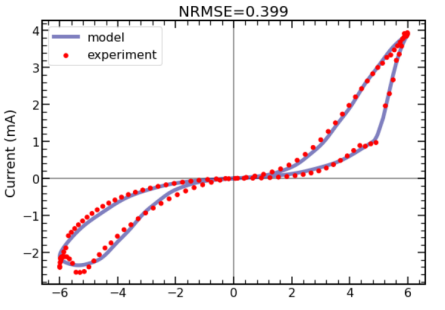
\includegraphics[scale=0.8]{latex_figure_a.png}
    \caption{a,}
    \label{fig:my_label}
\end{figure}
Fit of the $i-v$ characteristic calculated by the MHC Yakopcic model to the data obtained for the memristor device
developed in Skoltech, where the dynamics of a state variable
is described by a) the ordinary differential equation (4) and
b) the fractional differential equation (11).
i-v data are presented in Fig. 1. As mentioned above
we considered the equilibrium Nernst-potential of the
electrode to be zero, so that the electrochemical potential in Eqs. (8) and (11) is equal to the actual applied
voltage on the device. The corresponding fitting parameters are provided in Table I. As one can see, the
MHC-Yakopcic model fits very well to the experimental data with NRMSE = 0.401 for the fractional order
$\alpha = 0.697$. Remarkably enough, $\text{NRMSE} = 0.399$ when
the state variable evolves according to the ordinary differential equation, i.e., with $\alpha = 1$. In comparison, the
q-deformed memristor model recently reported in36 resulted in $\text{NRMSE} = 0.457$. The q-deformed model was
derived by taking into account gamma-distributed local
spatial inhomogeneities in the device structure. This provided a noticeable improvement in the fitting of the $i-v$ response of the same device under study here when
compared to the currently used existing model (i.e., the
Yakopcic model with MIM and Schottky electron transmission equations)36. However, as mentioned above,
the kinetics of electrode reactions in redox-based electrochemical metallization memory cells should be rather described by electron transfer theory. \par
The value of $\alpha = 0.697$ (Table I) in the fractional
derivative for the state variable equation indicates that
its dynamics does not evolve without prior knowledge of
all past information of its state or memory of its past.
This can be clearly illustrated by rewriting Eq. (21) as:
\begin{align}
   x_h^P (t_{n+1}) = \frac{h^\alpha}{\Gamma (\alpha + 1)} \biggl\{ F_n + \sum_{j=0}^{n-1} F_j \cdot b_{n-j} \biggr\} + ...,
\end{align}
which can be decoupled as the the sum of the immediate past of the state variable, and a memory trace41, represented by the second summation term, that contains information about all previous states of the device. \par
The magnitude of the memory trace term increases when $\alpha$ decreases further away from one, and when we are close to the actual instant t at which the variable is evaluated. At the limiting case of $\alpha = 1$, corresponding
to first-order integer derivative, the memory trace part
vanishes, and does not have any effect on the dynamics of
the state variable. Here, because $\alpha = 1$ we may speak of
an intrinsic memory embedded in our redox-based resistive memory device. Fractional dynamics are in fact very often observed in electrochemical devices and complex systems42–48. Indeed, a close inspection of Table I reveals that the fractional MHC-Yakopcic memristor model is practically insensitive to the input voltage $a_p, a_n \approx 0.$.
{\centering % Only center the section title
\section{Conclusion}
}
In this work we proposed a compact and accurate model for describing the electrical behavior of redoxbased resistive memory devices in which (i) the statecontrolled current-voltage equation is based on the MHC theory for electron transfer, and (ii) the dynamics of the
state variable is assumed to follow fractional time derivatives of order $\alpha (0 < \alpha < 1).$ 
For the numerical solution to the MHC integral we used the Gauss-Hermite quadrature method and for the fractional differential equation
of the state variable we used an Adams-type predictor corrector technique. Goodness of fit to the experimental data is evaluated in terms of NRMSE, and indicates superior capabilities of the proposed model when compared to recently reported ones. The obtained results, in connection to the electrochemical nature of the device under test, point out to necessity to take into consideration fractional dynamics when describing the $i-v$ characteristics of redox-based resistive memory devices. The fractional parameter can be viewed as an additional quantity representing the non-ideality, dissipative behavior of these devices.
\end{multicols}
\end{document}